\documentclass[a4paper]{article}
\usepackage{ucs}  % unicode
\usepackage[utf8x]{inputenc}
% \usepackage[T2A]{fontenc}
% \usepackage[bulgarian]{babel}
\usepackage{graphicx}
% \usepackage{fancyhdr}
% \usepackage{lastpage}
\usepackage{listings}
\usepackage{slashbox}
\usepackage{multirow}
\usepackage{wrapfig}
\usepackage{amsfonts}
\usepackage{amsmath, amsthm, amssymb}
% \usepackage{fancyvrb}
% \usepackage[usenames,dvipsnames]{color}
% \setlength{\headheight}{12.51453pt}

%\pagestyle{fancy}
%\fancyhead{}
%\fancyfoot{}

% \cfoot{\thepage\ от \pageref{LastPage}}

% \addto\captionsbulgarian{%
%   \def\abstractname{%
%     Цел на проекта} %\cyr\CYRA\cyrs\cyrt\cyrr\cyra\cyrk\cyrt}}%
% }

% Custom defines:
\def\definition{Definition:\ }
\def\la{\leftarrow}
\def\vars{\mathrm{Vars}}
\def\occ{\mathrm{Occ}}
\def\lub{\sqcup}
\def\xlub{\underline\lub}
\def\glb{\sqcap}
% \def\dc{bar baz}

% TODO remove colorlinks before printing
% \usepackage[unicode,colorlinks]{hyperref}   % this has to be the _last_ command in the preambule, or else - no work
% \hypersetup{urlcolor=blue}
% \hypersetup{citecolor=PineGreen}

\begin{document}

\newcommand{\aee}[1] {[[#1]]^\sharp}
\newcommand{\cc}[1] {\texttt{#1}}
\def\A {\mathcal{A}}
\def\N {\mathcal{N}}
\def\Neg {\mathrm{Neg}}
\def\Pos {\mathrm{Pos}}
\def\Vars {\mathrm{Vars}}
\def\Occ {\mathrm{Occ}}
\def\PP {\mathrm{ProgramPoints}}

\title{Static Program Analysis - Exercise 6}
\author{Iskren Ivov Chernev \\ tutorial group B}

\maketitle

\section{Solution}

\subsection*{Analysis}

Lets first define the carrier $ C $. It should store pairs of variables and
definition places. Because definition only occurs on edges, not program points,
for definition spots we shall use a pair of program points (we may also use
edges, which are triples of two program points and a label, but we are not
interested in the label). So the carrier is the set
$$
  C = \{(v, p_1, p_2)\ |\ v \in \Vars,\ p_1, p_2 \in \PP,\ \text{$ v $ is
  assigned in an edge from $ p_1 $ to $ p_2 $} \}
$$

Then the operation ``more precise than'' $ \sqsubseteq $ should be $ \subseteq
$, because the less triples we have, the more concrete the information is -- if
we have all triples it means we don't know anything about the last write
location, because it may be all of them.

Then $ \top $ is trivially all possible triples, and $ \bot $ is the empty set.

For combination of results from two paths we shall use union, because if
a variable was assigned on one edge on one path and on another edge on another
path than both are possible places for the last assignment. The initial value
at the begining of the program should be the empty set, because no assignments
were made. This means:

$$
  \A^\star[v] = \bigcup \{ \aee{\pi}\emptyset \ |\ \pi : start \longrightarrow^\star v \}
$$

Abstract edge effects are defined only for \texttt{assign} and \texttt{load}
operations, because the other don't change the variable bindings. Also, for the
first time, we will need the whole edge (including its endpoints) to define the
abstract edge effect.

\begin{eqnarray*}
  \aee{(u, x \leftarrow e, v)} D &=& \aee{(u, x \leftarrow M[e], v)}
  D \\ &=& D \setminus \{ (x, p_1, p_2)\ |\ p_1, p_2 \in \PP \} \cup \{ (x, u, v) \}
\end{eqnarray*}


\subsection*{Example}

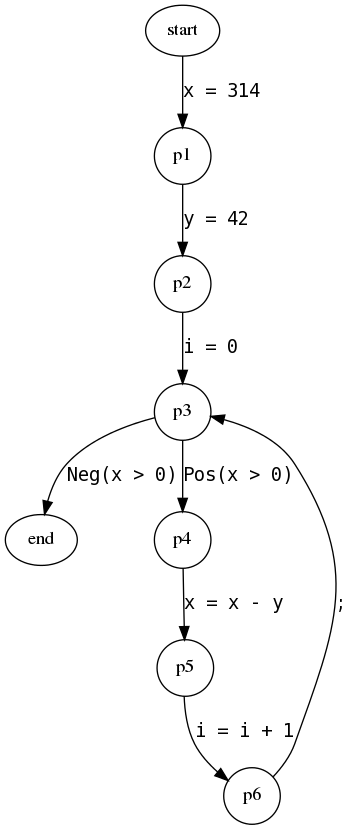
\includegraphics[scale=0.3]{6-1.png}

\begin{enumerate}
  \item Worklist : $ \{ start, p_1, p_2, p_3, p_4, p_5, p_6, end \}  $ \\
  extract point : $ start $ \\
  result : $ \{\} $, because this is the initial node, and no assignments are made \\
  push into worklist $ p_1 $, but it is already there.
  
  \item Worklist: $ \{ p_1, p_2, p_3, p_4, p_5, p_6, end \} $ \\
  extract point : $ p_1 $ \\
  expression : $ \aee{(start, x \leftarrow 314, p_1)} A[start] = \{\} \setminus \{ (x, u, v)\ |\ u, v \in \PP \} \cup \{ (x, start, p_1) \} $ \\
  result : $ A[p_1] = \{ (x, start, p_1) \} $ \\
  push into worklist $ p_2 $, but it is already there. 

  \item Worklist: $ \{ p_2, p_3, p_4, p_5, p_6, end \} $ \\
  extract point : $ p_2 $ \\
  expression : $ \aee{(p_1, y \leftarrow 42, p_2)} A[p_1] = \{ (x, start, p_1) \} \setminus \{ (y, u, v)\ |\ u, v \in \PP \} \cup \{ (y, p_1, p_2) \} $ \\
  result : $ A[p_2] = \{ (x, start, p_1), (y, p_1, p_2) \} $ \\
  push into worklkst $ p_3 $, but it is already there. 

  \item Worklist: $ \{ p_3, p_4, p_5, p_6, end \} $ \\
  extract point : $ p_3 $ \\
  expression : $ \aee{(p_2, i \leftarrow 0, p_3)} A[p_2] \cup \aee{(p_6, ;, p_3)} A[p_6] = \{ (x, start, p_1), (y, p_1, p_2) \} \setminus \{ (i, u, v)\ |\ u, v \in \PP \} \cup \{ (i, p_2, p_3) \} \cup \{\} $ \\
  result : $ A[p_3] = \{ (x, start, p_1), (y, p_1, p_2), (i, p_2, p_3) \} $ \\
  push into worklkst $ p_4 $ and $ end $, but they are already there.

  \item Worklist: $ \{ p_4, p_5, p_6, end \} $ \\
  extract point : $ p_4 $ \\
  expression : $ \aee{(p_3, \Pos(x > 0), p_4)} A[p_3] = \{ (x, start, p_1), (y, p_1, p_2), (i, p_2, p_3) \} $ \\
  result : $ A[p_4] = \{ (x, start, p_1), (y, p_1, p_2), (i, p_2, p_3) \} $ \\
  push into worklkst $ p_5 $, but it is already there. 

  \item Worklist: $ \{ p_5, p_6, end \} $ \\
  extract point : $ p_5 $ \\
  expression : $ \aee{(p_4, x \leftarrow x - y, p_5)} A[p_4] = \{ (x, start, p_1), (y, p_1, p_2), (i, p_2, p_3) \} \setminus \{ (x, u, v)\ |\ u, v \in \PP \} \cup \{ (x, p_4, p_5) \} $ \\
  result : $ A[p_5] = \{ (x, p_4, p_5), (y, p_1, p_2), (i, p_2, p_3) \} $ \\
  push into worklkst $ p_6 $, but they are already there.

  \item Worklist: $ \{ p_6, end \} $ \\
  extract point : $ p_6 $ \\
  expression : $ \aee{(p_5, i \leftarrow i + 1, p_6)} A[p_5] = \{ (x, p_4, p_5), (y, p_1, p_2), (i, p_2, p_3) \} \setminus \{ (i, u, v)\ |\ u, v \in \PP \} \cup \{ (i, p_5, p_6) \} $ \\
  result : $ A[p_6] = \{ (x, p_4, p_5), (y, p_1, p_2), (i, p_5, p_6) \} $ \\
  push into worklkst $ p_3 $.


  \item Worklist: $ \{ p_3, end \} $ \\
  extract point : $ p_3 $ \\
  expression : $ \aee{(p_2, i \leftarrow 0, p_3)} A[p_2] \cup \aee{(p_6, ;, p_3)} A[p_6] = \{ (x, start, p_1), (y, p_1, p_2) \} \setminus \{ (i, u, v)\ |\ u, v \in \PP \} \cup \{ (i, p_2, p_3) \} \cup \{ (x, p_4, p_5), (y, p_1, p_2), (i, p_5, p_6)  \} $ \\
  result : $ A[p_3] = \{ (x, start, p_1), (x, p_4, p_5), (y, p_1, p_2), (i, p_2, p_3), (i, p_5, p_6) \} $ \\
  push into worklkst $ p_4 $ and $ end $, $ end $ is already there.

  \item Worklist: $ \{ p_4, end \} $ \\
  extract point : $ p_4 $ \\
  expression : $ \aee{(p_3, \Pos(x > 0), p_4)} A[p_3] = \{ (x, start, p_1), (x, p_4, p_5), (y, p_1, p_2), (i, p_2, p_3), (i, p_5, p_6) \} $ \\
  result : $ A[p_4] = \{ (x, start, p_1), (x, p_4, p_5), (y, p_1, p_2), (i, p_2, p_3), (i, p_5, p_6) \} $ \\
  push into worklkst $ p_5 $.

  \item Worklist: $ \{ p_5, end \} $ \\
  extract point : $ p_5 $ \\
  expression : $ \aee{(p_4, x \leftarrow x - y, p_5)} A[p_4] = \{ (x, start, p_1), (x, p_4, p_5), (y, p_1, p_2), (i, p_2, p_3), (i, p_5, p_6) \} \setminus \{ (x, u, v)\ |\ u, v \in \PP \} \cup \{ (x, p_4, p_5) \} $ \\
  result : $ A[p_5] = \{ (x, p_4, p_5), (y, p_1, p_2), (i, p_2, p_3), (i, p_5, p_6) \} $ \\
  push into worklkst $ p_6 $.

  \item Worklist: $ \{ p_6, end \} $ \\
  extract point : $ p_6 $ \\
  expression : $ \aee{(p_5, i \leftarrow i + 1, p_6)} A[p_5] = \{ (x, p_4, p_5), (y, p_1, p_2), (i, p_2, p_3), (i, p_5, p_6) \} \setminus \{ (i, u, v)\ |\ u, v \in \PP \} \cup \{ (i, p_5, p_6) \} $ \\
  result : $ A[p_6] = \{ (x, p_4, p_5), (y, p_1, p_2), (i, p_5, p_6) \} $ \\
  the result is the same, so we do NOT push $ p_3 $ into worklist.

  \item Worklist: $ \{ end \} $ \\
  extract point : $ end $ \\
  expression : $ \aee{(p_3, \Neg(x > 0), end)} A[p_3] = \{ (x, start, p_1), (x, p_4, p_5), (y, p_1, p_2), (i, p_2, p_3), (i, p_5, p_6) \} $ \\
  result : $ A[end] = \{ (x, start, p_1), (x, p_4, p_5), (y, p_1, p_2), (i, p_2, p_3), (i, p_5, p_6) \} $ \\
  we don't have dependencies to push into worklist.


\end{enumerate}

\begin{tabular}{|r|l|}
  \hline
  point & value \\ \hline \hline
  $ A[start] $ & $ \{\} $ \\ \hline
  $ A[p_1] $ & $ \{ (x, start, p_1) \} $ \\ \hline
  $ A[p_2] $ & $ \{ (x, start, p_1), (y, p_1, p_2) \} $ \\ \hline
  $ A[p_3] $ & $ \{ (x, start, p_1), (x, p_4, p_5), (y, p_1, p_2), (i, p_2, p_3), (i, p_5, p_6) \} $ \\ \hline
  $ A[p_4] $ & $ \{ (x, start, p_1), (x, p_4, p_5), (y, p_1, p_2), (i, p_2, p_3), (i, p_5, p_6) \} $ \\ \hline
  $ A[p_5] $ & $ \{ (x, p_4, p_5), (y, p_1, p_2), (i, p_2, p_3), (i, p_5, p_6) \} $ \\ \hline
  $ A[p_6] $ & $ \{ (x, p_4, p_5), (y, p_1, p_2), (i, p_5, p_6) \} $ \\ \hline
  $ A[end] $ & $ \{ (x, start, p_1), (x, p_4, p_5), (y, p_1, p_2), (i, p_2, p_3), (i, p_5, p_6) \} $ \\ \hline
\end{tabular}

\end{document}
